
\section{Problem}  
To obtain necessary functionality, developers often use third-party libraries. Due to the complexity of current software systems, the dependency issue arises when the system depend on different and incompatible versions of the same library. This issue, called  `dependency hell'~\cite{wiki:hell} may break other dependencies or push the problem to another set of libraries.  We use an example to illustrate how the `dependency hell' causes a build error, how it is localized, how it is fixed in the next session.

%\noindent{\bf{Problem }}

\section{Example}


 \begin{figure}[!htb]
 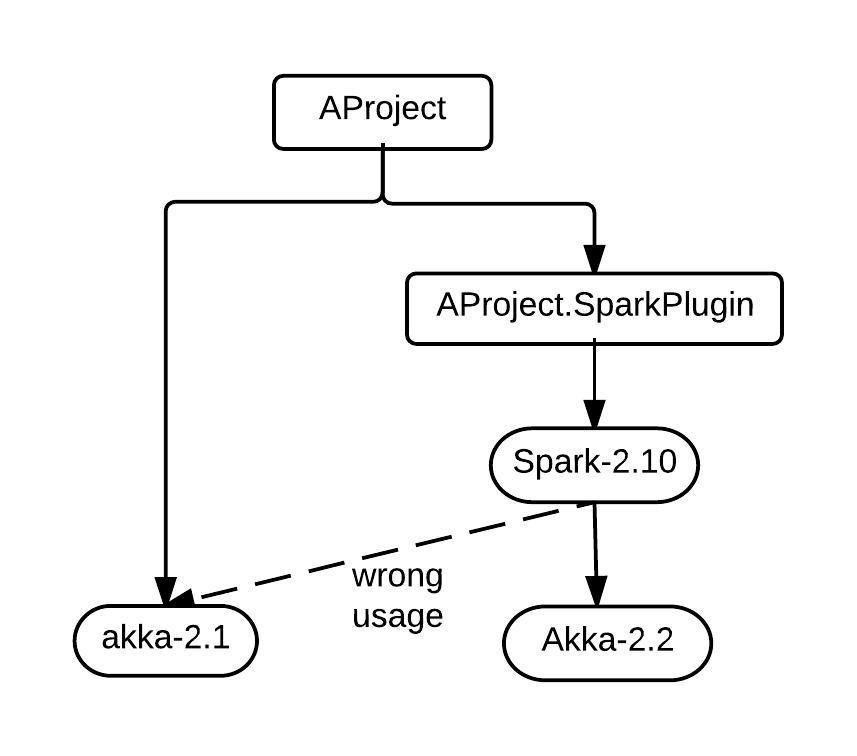
\includegraphics{akka.jpeg}
 \end{figure}
\noindent{\bf{What is the `dependency hell'?}}

\begin{figure}[!htb]
 \begin{minipage}{0.47\textwidth}
\scriptsize 
\begin{tabular}{@{}p{1\textwidth}} 
 \hline 
%  \multicolumn{1}{c}{(A) An inconsistent object name found by both Lancelot and \tool } \\ \hline
%  \vspace{-4mm}
%\begin{Verbatim}[commandchars=\\\{\}, tabsize=2]
% /* org.elasticsearch.action.DeleteRepositoryRequestBuilder */
%1.public String setName() \{
%2.  return setName;
%3.\}
%\end{Verbatim}
%\vspace{-4mm}
% \\ \hline
  \multicolumn{1}{c}{(A) Methods queried by user} \\ \hline
    \vspace{-4mm}
\begin{Verbatim}[commandchars=\\\{\}, tabsize=2]
/* org.apache.jena.json.JsonWriter */
1. public class JsonWriter implements JsonVisitor \{
2.  OutputStreamWriter writer;
3.  public void \bf{visit(JsonNumber jsonNumber)}  \{
4.   print(jsonNumber.value()) ; 
5.  \}
6.  public void \bf{visit(JsonBoolean jsonBoolean)} \{
7.   String x = Boolean.valueOf(jsonBoolean.value())?"true":"false"; 
8.   print(x);
9.  \}
10. private void \underline{print(Object s)} \{...
11.  writer.println(s);
12. \} ...\}
 \end{Verbatim}
   \vspace{-4mm}
  \\ \hline
   \multicolumn{1}{c}{(B) Callers of these two methods} \\ \hline
  \vspace{-4mm}
\begin{Verbatim}[commandchars=\\\{\}, tabsize=2]
 /* org.apache.accumulo.core.sync.SortedMapIterator */
1. public class JsonNumber extends JsonValue \{
2.  Format format;
3.  @Override
4.  public Object \underline{value()}
5.   \{ return format.getValue(value); \}
6.  @Override
7.  public void \uwave{visit(JsonVisitor visitor)}
8.   \{ visitor.visit(this) ; \}
9. \}
10. public class JsonBoolean extends JsonValue \{
11.  @Override
12.  public Object \underline{value()}
13.   \{ return value; \}
14.  @Override
15.  public void \uwave{visit(JsonVisitor visitor)}
16.   \{ visitor.visit(this) ; \}
17. \}
 /* Three of other 13 callers */
18. public class JsonFormatNumberHandler extends JsonHandler \{
19.  public static void \uwave{printNumber(JsonNumber jNum)} \{
20.   JsonWriter w = new JsonWriter(output);
21.   jNum.setFormat(format);
22.   w.visit(jNum);
23. \} ...\}
24. public class JSONNumberOptional \{
25.  JsonBoolean jBool; 
26.  JsonNumber left, right;
27.  public static void \uwave{recordOptional()} \{
28.   JsonWriter w = new JsonWriter(output);
29.   w.visit(left);
30.   w.visit(jBool);
31.   w.visit(right);
32. \} ...\}
33. public class JSON \{
34.  public static void \uwave{write(JsonValue jValue)} \{
35.   JsonWriter w = new JsonWriter(output);
36.   w.visit(jValue);
37. \} ...\}
\end{Verbatim}
\vspace{-4mm}
 \\ \hline
\end{tabular} 
\caption{Example of suggested elements given a set of interest}
\label{fig:compare}
\end{minipage}
\end{figure}



%%%%%%%Usage pattern example %%%%%%%

%
%\begin{figure}[!htb]
% \begin{minipage}{0.47\textwidth}
%\scriptsize 
%\begin{tabular}{@{}p{1\textwidth}} 
% \hline 
% \multicolumn{1}{c}{(A) An inconsistent object name found by both Lancelot and \tool } \\ \hline
%  \vspace{-4mm}
%\begin{Verbatim}[commandchars=\\\{\}, tabsize=2]
% /* org.elasticsearch.action.delete.DeleteRepositoryRequestBuilder */
%1.public String setName() \{
%2.  return setName;
%3.\}
%\end{Verbatim}
%\vspace{-4mm}
% \\ \hline
%  \multicolumn{1}{c}{(B) A naming bug from Lancelot} \\ \hline
%   \vspace{-4mm}
%\begin{Verbatim}[commandchars=\\\{\}, tabsize=2]
%/* org.elasticsearch.action.termvector.TermVectorFields */
%1.public void size(int size) \{
%2.  if (size <= 0) 
%3.   throw new legalArgumentException("Size must be positive"); 
%4.  this.size = size;
%5.\}
% \end{Verbatim}
% Lancelot said: Methods with this name never return void.
% \vspace{-4mm}
%  \\ \hline
%\end{tabular} 
%\caption{Name Checker comparison}
%\label{fig:compare}
%\end{minipage}
%\end{figure}
 

We illustrate the building error caused by `dependency hell' in a Maven project shown in Figure~\ref{fig:shifu}. As shown in part A, the parent project uses akka 2.1.1 to initialize \codefont{ActorRef} (underline) by creating a new \codefont{Props} object. The developer Alice is asked to implement a new sub-module named as SparkPlugin using Spark framework. Without knowing that Spark is dependent on akka-2.2.3, she implements the entire sub-module with Spark-1.0.0, writes the tests, and fully tests the single submodule before integrating with the parent project. However, she encounters the building error shown as part (C) (The complete building error is shown at~\cite{shifu}). 

\noindent{\bf{How to localize `dependency hell'?}} 

Starting from the \codefont{NoSuchMethodException}, she investigates the \codefont{akka.remote.RemoteActorRefProvider.<init>}  in akka-2.2.3 as declared in Spark's pom.xml and finds the static \codefont{Props.create} method shown in part (D). Alice get confused on the \codefont{NoSuchMethodException} and she has to use step-by-step debugging. She finally notices that the maven build system mistakenly uses akka-2.1.1 inherited from parent project, rather than the akka-2.2.3 that is required for Spark library. 

\noindent{\bf{How to fix `dependency hell'?}}

  Alice has several options to fix this bug as below:
\begin{enumerate}
\item change akka version in parent class to 2.2+, which is not feasible as the parent project heavily uses akka and it requires tremendous effort for upgrading.
\item  exclude all transitive dependencies inherited from parent project with the feature provided by Maven 3.2.2+~\cite{maven:note}, aiming to resolve dependency hell~\cite{maven:hell}. This approach is not feasible as well because SparkPlugin itself relies on the parent projects and Alice has to re-import all dependencies that the submodule uses.
\item include both akka versions and enforce Spark to use akka-2.2.3. This approach is similar to the well-known side-by-side  mechanism used in NIX package manager for Linux-based system~\cite{nix}. This might fix the build error, but Alice is concerned that compiling both versions might increase the building time of the entire system. 
\item exclude akka-2.1.1 from the dependency declaration of Spark-1.0.0. Alice decides to use this solution as it won't have ripple effect on the rest of the system.
\end{enumerate}


%To ensure that there does not exist any other transitive dependency that causes dependency hell, she tries maven-enforcer plugin which have the rule to ban all transitive dependencies~\cite{maven:enforcer}, yet the plugin outputs more than 100 conflicts. Alice gives up to kill all conflicts as (1) It is costly to exclude all conflicts, (2) it makes the maven hard to maintain, and (3) most of them might not be harmful for the system. 

Using this example, we illustrate that  it is not easy to  localize dependency hell without knowing the entire dependency graph and it can be error-prone when trying to fix the error.

\section{Approach}

%There are some well-known solutions to this problem, they either ask developers to manually exclude all the transitive dependencies for a dependency (Solution 2) or include multiple versions in a side-by-side manner (Solution 3). Neither of them are perfect as described in the previous session. 

We propose an approach to check compatibility on the interfaces that use different versions for the same libraries, which has the possibility to introduce `dependency hell'. Instead of strict backward compatibility checker for the entire class~\cite{Welsch:backward12}, we regard it as safe if the used API is compatible for the other version in the current usage context. We make this trade-off because developers often embrace changes, making multiple versions incompatible to each other~\cite{bogart:backward}. To save build time and space,  we include multiple versions of the files from the same library only if they are incompatible with each other, instead of maintaining multiple versions for the same library at the same time. To save time for analysis, we only consider the API calls when it has the possibility to generate `dependency hell', since there is no need to check the dependency issue if the libraries are consistent used in the system with a single version.

